\documentclass{article}
\title{Single-cell data analysis in the browser}
\usepackage{authblk}
\usepackage{hyperref}
\usepackage{graphicx}
\usepackage{multirow}
\usepackage{color}

\author[1]{Aaron Lun}
\affil[1]{Genentech, Inc. South San Francisco, CA}
\author[1]{Jayaram Kancherla}

\begin{document}
\maketitle

\newcommand{\code}[1]{\texttt{#1}}
\newcommand{\jay}[1]{\textcolor{red}{#1}}

\section{Introduction}

Modern web browsers are sophisticated pieces of software responsible for rendering, scripting, networking, data storage and more.
New web technologies such as WebAssembly \cite{haas2017bringing} have greatly enhanced browsers' capabilities for intensive computation,
providing new opportunities to repurpose the browser as an interactive data analysis tool.
The idea is to use the browser itself to perform statistical and computational analyses directly on the user's machine, i.e., ``client-side compute". 
Those analysis results can then be rendered on a web page for convenient visualization and exploration within a familiar interface.

This paradigm of client-side compute in the browser has several advantages over the traditional model of server-side data analysis.
Most obviously, we do not need a backend server to perform any of the calculations, simplifying deployment and reducing costs.
As the entire analysis is performed on the client machine, we avoid any data transfer - this reduces latency in the user interface and circumvents concerns over data ownership and privacy.
Finally, we do not require installation of any data analysis environments like R or Python, ensuring that the analyses are accessible to audiences of varying computational skill.

A modest body of prior work exists to realize these client-side benefits for bioinformatics data analysis.
For example, the BioJS registry contains several Javascript components for handling biological data \cite{gomez2013biojs}, many of which focus on DNA and protein sequence analysis.
The \code{BrowserGenome.org} application performs read alignment and transcript quantification for RNA sequencing data \cite{schmid2015browsergenome},
while the \code{ubit2} application analyzes single-cell quantitative polymerase chain reaction datasets \cite{fan2017ubit2};
both use Javascript implementations of the relevant algorithms to run in the browser.
However, these are exceptions to the rule; most bioinformatics web applications only use the browser to visualize results that were computed elsewhere,
e.g., \cite{megill2021cellxgene}, \cite{chelaru2014epiviz}, (\jay{JAY TO PROVIDE EXAMPLES}) and every R/Shiny application ever.
After all, Javascript is not widely recognized as a language for data science, nor is it particularly efficient for such tasks.

The client-side paradigm is especially appealing for single-cell genomics due to the exploratory nature of its data analysis.
Most use cases for single-cell sequencing involve identifying new cell subpopulations or states from heterogeneous biological samples \cite{stegle2015computational},
which requires several iterations of data analysis, visualization and interpretation.
If the compute could be performed in the browser, the results could be immediately rendered on a web page for a seamless transition between analysis and interactive exploration.
However, this is complicated by the size of the datasets, each of which involves tens of thousands of genes and up to millions of cells;
and the paucity of browser-compatible implementations of relevant algorithms, most of which are written in R or Python.

We present \code{kana}, a web application for single-cell RNA-seq (scRNA-seq) data analysis inside the browser.
\code{kana} provides a streamlined one-click workflow for all steps in a typical scRNA-seq analysis \cite{amezquita2020orchestrating}, 
starting from a count matrix and finishing with marker detection.
Users can interactively explore the low-dimensional embeddings, clusterings and marker genes in an intuitive graphical interface that encourages iterative re-analysis.
Once finished, users can save their analysis and results for later examination or sharing with collaborators.
By using technologies like WebAssembly and web workers, we achieve high-performance compute for datasets containing hundreds of thousands of cells.

The \code{kana} application is available at \url{https://www.jkanche.com/kana}.
Developers can set up their own deployments by following the instructions at \url{https://github.com/jkanche/kana}.

\section{Application overview}

Given a scRNA-seq dataset, \code{kana} implements a routine analysis with the steps listed below.
We will not discuss the statistical and scientific rationale behind each step in much detail as this has been covered elsewhere \cite{oscabook}.

\begin{enumerate}
\item We import a gene-by-cell count matrix from the user's machine, typically in the form of Matrix Market files such as those produced by the Cellranger pipeline.
HDF5 files are also supported, using either the 10X HDF5 feature barcode matrix format or as H5AD files.
\item We compute common quality control (QC) metrics such as the total count, number of detected genes and proportion of mitochondrial counts.
Low-quality cells are defined as those cells with outlier values for any of these metrics; these are filtered out from subsequent steps.
\item We perform scaling normalization based on the library size to remove cell-specific biases.
This is followed by a log-transformation to obtain a matrix of log-normalized expression values.
\item We fit a LOWESS trend \cite{cleveland1979robust} to the per-gene variances with respect to the means, computed from the log-expression values.
We sort on the residuals to define a subset of highly variable genes (HVGs). 
\item We perform principal components analysis (PCA) on the log-expression matrix with the subset of HVGs.
This yields a few top PCs that capture the heterogeneity of the data in a compressed and denoised form.
\item We apply clustering techniques on the top PCs to generate discrete subpopulations.
Specifically, we apply multi-level (i.e., ``louvain'') community detection on a shared nearest neighbor (SNN) graph where each cell is a node and edges connect neighboring cells.
Each cluster is characterized through differential expression analyses to detect its marker genes.
\item We perform further dimensionality reduction on the top PCs to obtain two-dimensional embeddings for visualization. 
This includes the usual t-distributed stochastic neighbor embedding (t-SNE) and uniform manifold approximation and projection (UMAP) \cite{maaten2014accelerating,mcinnes2018umap}.
\end{enumerate}

At each step, users can easily customize key parameters (Figure \ref{screenshot:analysis}).
For example, we can adjust the QC thresholds, the number of HVGs and top PCs, the granularity of the clustering, and more. 
Iterative refinements to the parameters are encouraged in \code{kana}, as the application tracks dependencies between steps to enable efficient re-analysis.
Specifically, when parameters are modified for any step, all subsequent steps are automatically re-executed to propagate the change to downstream results.
Conversely, \code{kana} does not rerun any steps upstream of the change to avoid unnecessary recomputation and reduce latency.

\begin{figure}[htbp]
\begin{center}
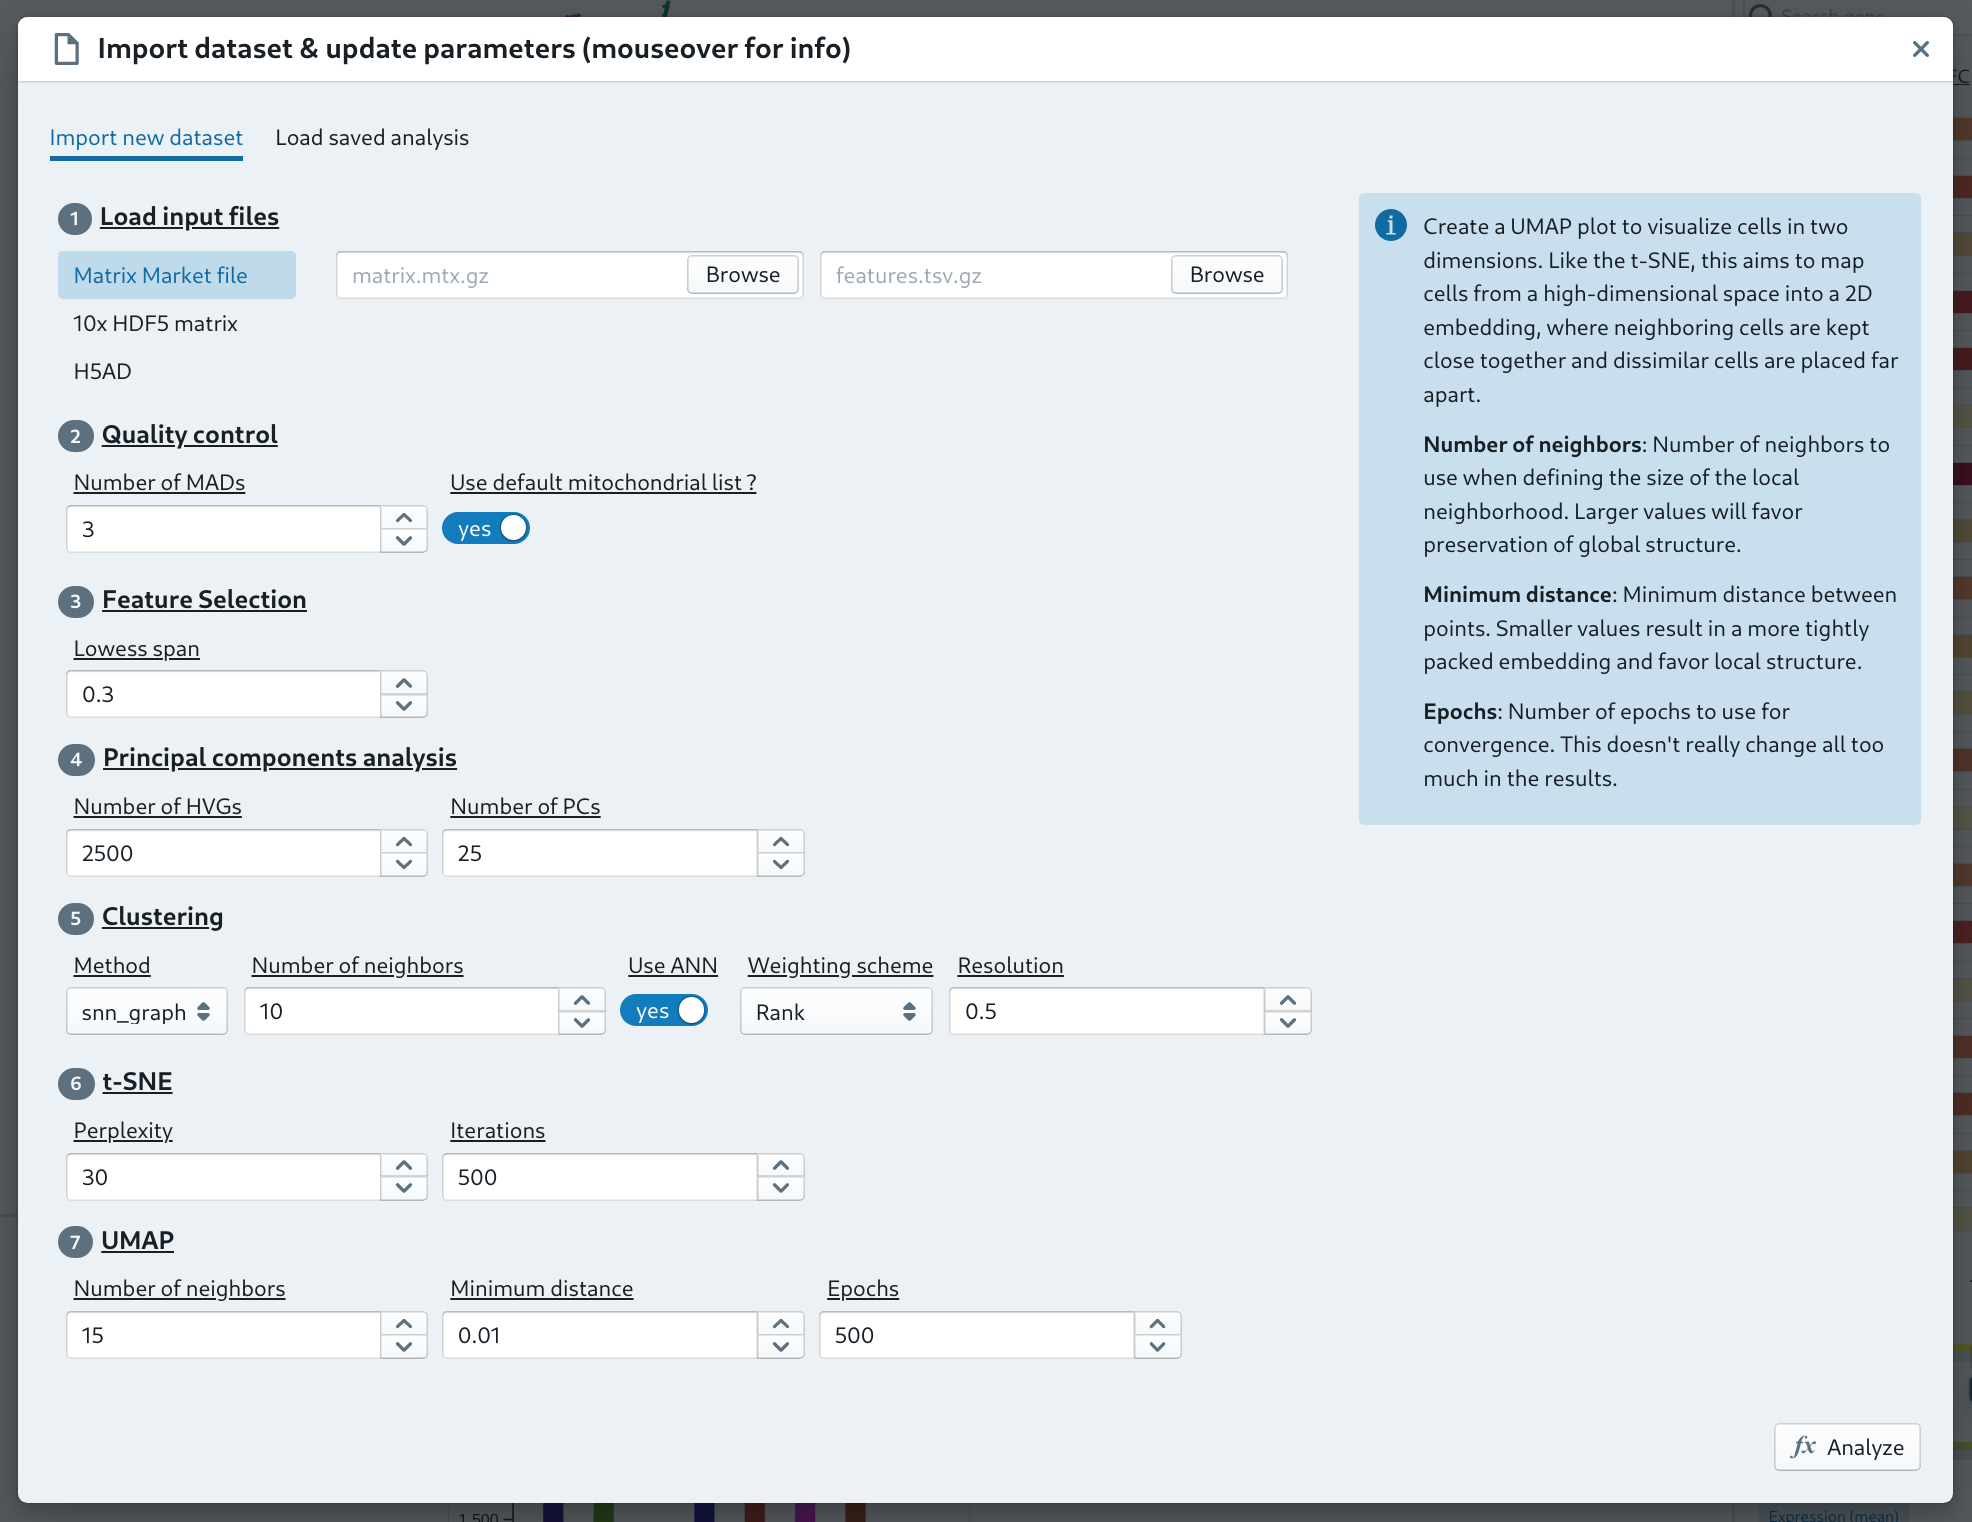
\includegraphics[width=\textwidth]{screenshots/analysis.png}
\end{center}
\caption{Screenshot showing the analysis configuration panel in the \code{kana} application.
Clicking ``Analyze" will perform the entire analysis.}
\label{screenshot:analysis}
\end{figure}

Once each step of the analysis is complete, \code{kana} visualizes its results in a multi-panel layout (Figure \ref{screenshot:results}).
One panel contains a scatter plot for the low-dimensional embeddings, where each cell is a point that is colored by cluster identity or gene expression.
Another panel contains a table of marker statistics for a selected cluster, where potential marker genes are ranked and filtered according to the magnitude of upregulation over other clusters.
We also have a gallery to visualize miscellaneous details such as the distribution of QC metrics.

\begin{figure}[htbp]
\begin{center}
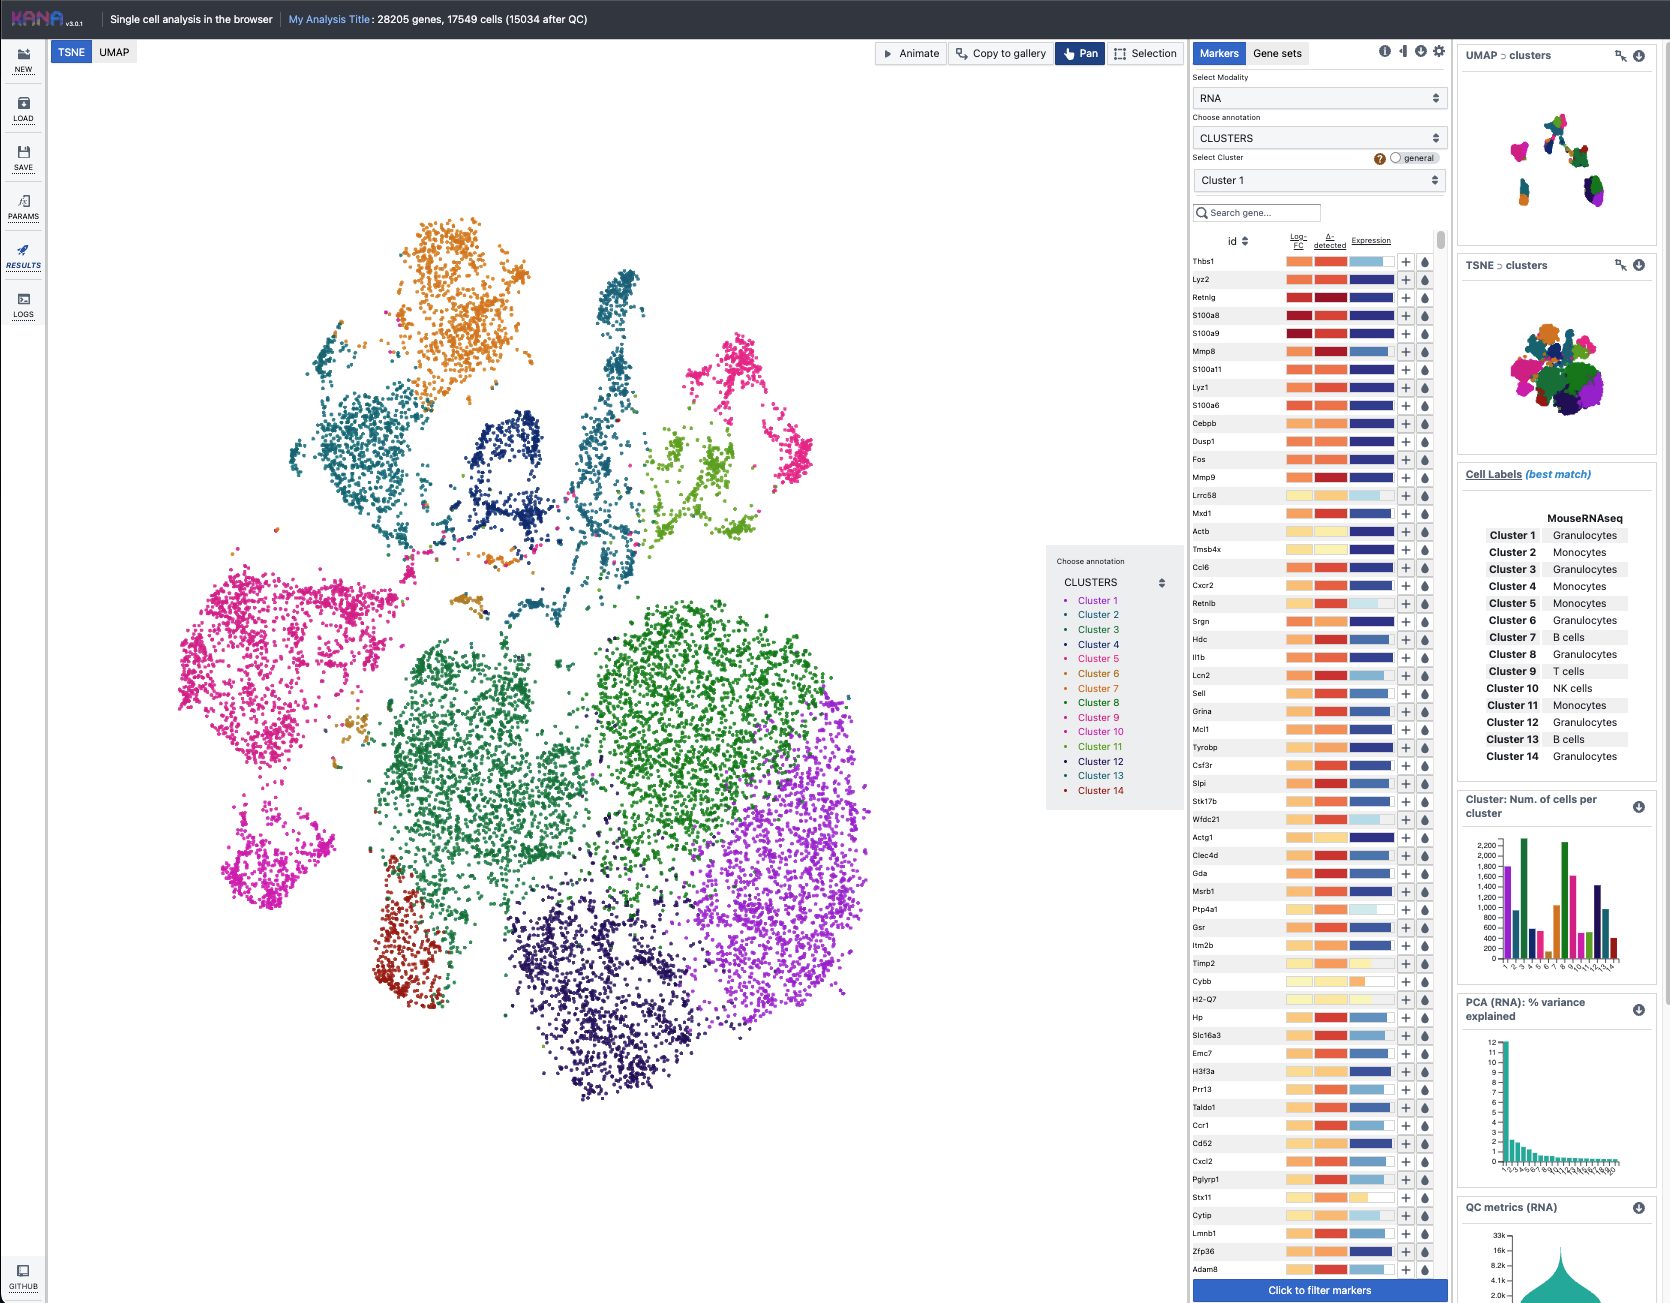
\includegraphics[width=\textwidth]{screenshots/results.png}
\end{center}
\caption{Screenshot showing the multi-panel layout for results in the \code{kana} application.
The top-left panel is used for the low-dimensional embeddings,
the right panel contains the marker table for a selected cluster,
and the bottom-left panel contains a gallery of miscellaneous plots.}
\label{screenshot:results}
\end{figure}

Finally, users can export the analysis parameters and results for later inspection.
The exported analysis can be quickly reloaded in a new browser session, allowing users to view the results without repeating the computation.

\section{Client-side computation}

\subsection{Efficient compute with WebAssembly}

WebAssembly (Wasm) is an instruction format that provides a web-executable compilation target for languages like C/C++, Go and Rust.
This allows us to turn the browser into a compute engine by integrating existing scientific libraries for bioinformatics data analysis -
see the biowasm project (\url{https://github.com/biowasm/biowasm}) for previous work in this direction.
For \code{kana}, we collected C++ implementations of the algorithms required for each step:

\begin{itemize}
\item The \code{tatami} library (\url{https://github.com/LTLA/tatami}) provides an abstract interface to different matrix classes, 
based on similar ideas in the \code{beachmat} package \cite{lun2018beachmat}. 
In addition to the usual dense and sparse representations, \code{tatami} also supports the delayed operations implemented in the \code{DelayedArray} package \cite{delayedarray}.
This allows the creation of QC-filtered and log-normalized matrices without any duplication of expression data.
\item The \code{CppWeightedLowess} library (\url{https://github.com/LTLA/CppWeightedLowess}) contains a C++ port of the \code{weightedLowess} function from the \code{limma} package \cite{ritchie2015limma}.
This function is, in turn, based on the LOWESS algorithm \cite{cleveland1979robust} implemented in R's \code{lowess} function, 
modified with the ability to consider weights in the span calculations.
\item The \code{CppIrlba} library (\url{https://github.com/LTLA/CppIrlba}) library contains a C++ port of the IRLBA algorithm \cite{baglama2005augmented} to efficiently obtain the top PCs from an input matrix.
This is based on the C code in the \code{irlba} package \cite{irlba} with some refactoring to eliminate R-specific dependencies.
In particular, we now rely on the Eigen library \cite{eigenweb} for matrix operations.
%\item The \code{CppKmeans} library (\url{https://github.com/LTLA/CppKmeans}) contains C++ implementations of the Hartigan-Wong \cite{hartiganwong} and Lloyd algorithms \cite{lloyd} for k-means clustering.
%In particular, the Hartigan-Wong implementation was translated from the Fortran code used by R's \code{kmeans} function.
\item The \code{knncolle} library (\url{https://github.com/LTLA/knncolle}) wraps several nearest neighbor detection algorithms in a consistent interface for interchangeable use.
This includes exact methods like vantage point tree search \cite{yianilos1993data} as well as approximate methods like Annoy \cite{annoy}.
It is equivalent to the \code{BiocNeighbors} package from Bioconductor \cite{biocneighbors}.
\item The \code{libscran} library (\url{https://github.com/LTLA/libscran}) implements high-level methods for scRNA-seq data analysis, ranging from quality control to clustering.
The code here originates from the \code{scran}, \code{scuttle} and \code{scater} packages \cite{lun2016step,lun2017scater} bundled together into a single C++ library for convenience. 
This library relies on the \code{igraph} C library \cite{csardi2006igraph} for community detection from the SNN graph.
\item The \code{qdtsne} library (\url{https://github.com/LTLA/qdtsne}) contains a C++ implementation of the Barnes-Hut t-SNE algorithm \cite{maaten2014accelerating}.
This is mostly a refactored version of the code in the \code{Rtsne} package \cite{rtsne}.
Some additional optimizations have been applied to improve scalability.
\item The \code{umappp} library (\url{https://github.com/LTLA/umappp}) contains a C++ implementation of the UMAP algorithm \cite{mcinnes2018umap}.
This is largely derived from code in the \code{uwot} package \cite{uwot}.
\end{itemize}

We created the \code{scran.js} library (\url{https://github.com/jkanche/scran.js}) to provide Javascript bindings to these C++ libraries.
Specifically, we compiled our C++ code to Wasm using the Emscripten toolchain \cite{zakai2011emscripten},
allowing \code{kana} to perform scRNA-seq-related calculations from Javascript by calling \code{scran.js} functions.
The same library can also be used in other web applications via a standard NPM installation (\url{https://www.npmjs.com/package/scran.js}),
or outside the browser if a suitable Wasm runtime environment is available.

To evaluate the efficiency of our Wasm strategy, 
we compared a \code{kana} analysis in the browser to that of a native executable compiled from the same C++ libraries (\url{https://github.com/LTLA/scran-cli}).
We analyzed several public scRNA-seq datasets (Table \ref{tab:datasets}) using the default \code{kana} parameters for both approaches, i.e.,
QC filtering to 3 MADs from the median;
PCA on the top 2500 HVGs to obtain the top 25 PCs;
SNN graph construction with 10 neighbors and multi-level community detection at a resolution of 0.5;
t-SNE with a perplexity of 30;
and UMAP with 15 neighbors and a minimum distance of 0.01.
We collected timings on \jay{Jay's Linux laptop} using 8 web workers for \code{kana} (see below) and 8 threads for the executable.
For convenience, we ran the \code{kana} timings in batch using Puppeteer (\url{https://github.com/puppeteer/puppeteer}) to control a headless Chrome browser (\jay{vXXXX}).

\begin{table}
\caption{Collection of scRNA-seq datasets used for testing.}
\label{tab:datasets}
\begin{center}
\makebox[\textwidth][c]{
\begin{tabular}{l l l l r}
\hline
Study & Species & Tissue & Technology & \multicolumn{1}{c}{Number of cells} \\
\hline
Zeisel \emph{et al.} (2015) \cite{zeisel2015cell} & Mouse & Brain & STRT-seq & 3005 \\
Paul \emph{et al.} (2015) \cite{paul2015transcriptional} & Mouse & Bone marrow & MARS-seq & 10368 \\
Bach \emph{et al.} (2017) \cite{bach2017differentiation} & Mouse & Mammary gland & 10x Genomics & 25806 \\
Ernst \emph{et al.} (2019) \cite{ernst2019staged} & Mouse & Spermatogonia & 10x Genomics & 68937 \\
Bacher \emph{et al.} (2020) \cite{bacher2020low} & Human & T cells & 10x Genomics & 104417 \\
Zilionis \emph{et al.} (2019) \cite{zilionis2019single} & Human & Lung & 10x Genomics & 173954 \\
\hline
\end{tabular}
}
\end{center}
\end{table}

%Our results indicate that \code{kana} analyses took approximately 20-30\% more time compared to the native executable (Table \ref{tab:times}).
%This is consistent with Wasm's promise of near-native execution and is comparable to existing benchmarking results \cite{jangda2019not}.
%The performance gap can be attributed to the overhead of the Wasm runtime environment in the browser
%and the differences in optimization levels of the compiler toolchains (Emscripten/Clang for Wasm, GCC for the executable).
%We note that there are still some opportunities for optimization in our Wasm compilation process -

\begin{table}
\caption{Analysis run times for several datasets with \code{kana} or a native executable.
Values are reported in seconds with standard errors from 3 runs.}
\label{tab:times}
\begin{center}
\begin{tabular}{l r r r}
\hline
Dataset & \multicolumn{1}{c}{Number of cells} & \multicolumn{1}{c}{\code{kana}} & \multicolumn{1}{c}{Native} \\
\hline
Zeisel   & 3005   &  $\pm$ & $\pm$ \\
Paul     & 10368  &  $\pm$ & $\pm$ \\
Bach     & 25806  &  $\pm$ & $\pm$ \\
Ernst    & 68937  &  $\pm$ & $\pm$ \\
Bacher   & 104417 &  $\pm$ & $\pm$ \\
Zilionis & 173954 &  $\pm$ & $\pm$ \\
\hline
\end{tabular}
\end{center}
\end{table}

\subsection{Parallelization with web workers}

Web workers provide a simple mechanism for parallelization inside the browser.
In \code{kana}, a web worker is used to run the compute-intensive analysis in its own thread so that the application's main thread is free to respond to user interaction.
However, we also use web workers to parallelize the computations within some of the analysis steps by compiling our C++ code with PThreads support.
This implements POSIX threads as web workers for transparent parallelization across genes or cells during calculation of QC metrics, nearest neighbor detection and marker scoring.
In addition, we parallelize across steps by manually creating a separate web worker to execute the t-SNE, UMAP and clustering steps, which are independent of each other and can run concurrently.

A minor complication with PThreads is that we need to enable cross-origin isolation on the \code{kana} site.
Briefly, this is a security measure that prevents inappropriate data access from malicious scripts in the same browsing context.
Once cross-origin isolated, the site is permitted to use the \code{SharedArrayBuffer} for copy-free transfer of data between web workers.
To achieve this, we need to serve the \code{kana} assets with the appropriate cross-origin headers - specifically, the embedder and opener policies.
However, this may not always be possible, e.g., when hosting on institutional sites or public sites such as GitHub Pages.
Instead, we use a service worker to cache and re-serve \code{kana} with the correct headers,
ensuring that it can be easily deployed in a range of hosting environments.

As a matter of etiquette, we limit \code{kana} to two-thirds of the available threads at maximum utilization.
The intention is to leave enough resources available for other activities to pass the time while waiting for the analysis to finish.

\subsection{Creating layered sparse matrices}

To reduce memory usage for large single-cell count matrices, we use a ``layered matrix" approach that splits the input matrix by row into 3 sparse submatrices.
The first, second and third submatrices contain data for genes where all non-zero counts can fit into 8-bit, 16-bit and 32-bit unsigned integers, respectively.
This improves memory efficiency as large datasets generally have low sequencing coverage;
most counts can be represented as 8-bit integers to save space, leaving a few high-abundance genes to be stored in the submatrices with larger integer types.
A similar strategy is applied to row indices for non-zero elements in a sparse matrix, where most datasets have fewer than 60,000 genes and can be accommodated with 16-bit integers.
This gives a theoretical usage of 3 bytes per non-zero element, e.g., a dataset with 30,000 genes and 100,000 cells at 5\% density requires around 500 MB of memory in this data structure.

The layered matrix representation is implemented through the delayed binding mechanism in \code{tatami}.
Specifically, we create the individual sparse submatrices and then create an abstract represention of the full matrix where the submatrices are combined by row.
This preserves the memory-efficient representation while presenting an interface that mimics that of a single matrix.
The layered representation can then be seamlessly used with all existing code compatible with the \code{tatami} interface.
(Note that the genes are permuted from their supplied order, which requires some extra attention in downstream analyses.)

We evaluated the performance of this data structure by recording the memory usage of the analyses in Table \ref{tab:times}.

% Need to add memory usage here.
\begin{table}
\caption{Memory usage of \code{kana} during the analysis of several datasets.
We report the memory usage immediately after the count matrix is loaded, as well as peak usage throughout the entire analysis.
Values are reported in megabytes.}
\label{tab:memory}
\begin{center}
\begin{tabular}{l r r r}
\hline
Dataset & \multicolumn{1}{c}{Number of cells} & \multicolumn{1}{c}{\code{kana}} & \multicolumn{1}{c}{Native} \\
\hline
Zeisel   & 3005   &  & \\
Paul     & 10368  &  & \\
Bach     & 25806  &  & \\
Ernst    & 68937  &  & \\
Bacher   & 104417 &  & \\
Zilionis & 173954 &  & \\
\hline
\end{tabular}
\end{center}
\end{table}

\section{User interface concepts}

\subsection{Interlinked graphics}

Different panels of the \code{kana} application (Figure \ref{screenshot:results}) can share information with each other to facilitate interactive exploration of the dataset and analysis results.
For example, we can color the embeddings according to the expression of a gene selected from the marker table.
Upon selection, \code{kana} retrieves the log-normalized expression values for that gene from the sparse matrix and passes this data to the scatter plot for coloring.
Users can also adjust the color gradient to improve contrast and highlight differences at particular ranges of expression.

A more complex example involves the detection of new marker genes for a custom selection of cells.
Users can create a custom selection by brushing on regions of interest in the embedding panel.
If this selection is saved, \code{kana} will perform a differential expression analysis to detect upregulation inside the selection compared to all other cells.
Statistics for each gene are then shown in the marker table for examination.
Each custom selection and its statistics are treated as part of the analysis state and are saved during export.

Users can also save specific views of the embeddings into the gallery for later perusal (\jay{cite CIRROCUMULUS}).
This is useful for simultaneously viewing multiple plots colored by different marker genes to characterize complex populations.

\subsection{Progressive rendering}

Each result is immediately rendered on the interface once the corresponding analysis step is complete.
For example, the distribution of QC metrics appear once the QC step is finished, followed by the plot of the percentage of variance explained once the PCA is done, and so on.
This improves application performance by avoiding the rendering bottleneck that would otherwise occur if all plots were drawn at once. 
It also serves as a visual progress indicator and improves the user experience by showing meaningful content as soon as possible.

The marker table is a more subtle example of progressive rendering.
Only the genes in the current view of the table are rendered, with the remaining visual elements being dynamically created as the user scrolls up or down to see other genes in the ranking.
This ensures that we do not waste time rendering tens of thousands of rows when only the top few are likely to be viewed.

Given that \code{kana} is computing the embeddings in the background, we can actively monitor the change in the coordinates for each cell across t-SNE iterations or UMAP epochs.
We do so by extracting the coordinates at regular intervals and rendering them on the embedding panel with WebGL,
effectively creating an animation of the embedding as it is refined over time.
This is mostly present for entertainment value but may provide some educational insights into the process of creating the embeddings (e.g., early exaggeration for t-SNE).

% \subsection{Accelerated graphics with WebGL}
% 
% WebGL is a Javascript application programming interface (API) for efficient rendering of interactive graphics in the browser.
% It does so by leveraging the client device's graphics processing unit (GPU) to accelerate the creation of images from data and shader instructions.
% \code{kana} uses the WebGL API to quickly visualize the dimensionality reduction results for hundreds of thousands of cells, each of which must be rendered as a separate point.
% For the animations across t-SNE/UMAP iterations, we observed a frame rate of \jay{XX $\pm$ XX} frames per second (FPS) when using WebGL 
% compared to the \jay{YY $\pm$ YY} FPS with the standard canvas API.
% This improved performance with WebGL contributes to a more comfortable user experience when interacting with the dimensionality reduction plot in \code{kana},
% both in terms of smooth animations across iterations as well as smooth transitions when panning, zooming or selecting points.

\subsection{Exporting and reloading}

Users can choose to export their analyses to the browser's cache via its in-built \code{IndexedDB} database system.
This dumps the analysis state (i.e., parameters and results) into a Gzip-compressed JSON inside the cache, along with the input data files.
Users can then reload their analysis in a new browser session without needing to keep track of any files.
Moreover, \code{kana} will attempt to deduplicate input files in the cache based on the file name, size and MD5 checksum.
This reduces disk usage when storing multiple analysis states for the same dataset. 

Alternatively, users may export the analysis state to a file that is downloaded to their machine.
This creates a single binary file containing the Gzip-compressed analysis state and the embedded input files.
Supplying this file to \code{kana} will then restore the previous analysis in the same manner as using the browser cache.
The benefit of this approach is that files exported by one user can be reloaded by other users on different machines,
allowing users to easily share their analyses with each other by simply transferring the relevant files.
In fact, computationally savvy users can even parse the \code{kana}-exported file in other programming frameworks (e.g., R, Python) for custom processing.

\section{Discussion}

Single-cell data analysis on the client is not a particularly novel concept.
In many cases, the dataset already lives on the user's machine, so this is a natural place to perform the analysis with the tool of choice (typically R or Python).
\code{kana}'s key innovation lies in its use of modern web technologies to perform the analysis directly in the browser.
This eliminates the difficulties of software installation and makes the analysis accessible to a non-programming audience.
At the same time, we retain all the benefits of client-side operations.
Specifically, our availability only depends on the client device, not on a backend server;
there is no latency from transferring data or results across a network;
ownership of the dataset clearly remains with the user, avoiding issues with data privacy and associated regulations;
and compute time is cheap, if not effectively free.

Client-side compute has interesting scalability characteristics compared to a traditional backend approach.
Most obviously, we are constrained by the computational resources available on the client machine,
which can vary from modest (e.g., most laptops) to extremely basic (e.g., mobile devices).
This limits the size of any single dataset that can be analyzed by a particular client.
However, in other respects, client-side compute is more scalable than backend compute;
the former automatically distributes analyses of many datasets across any number of machines at no cost and with no configuration.
This is especially relevant for web applications like \code{kana} where the maintainers would otherwise be responsible for provisioning backend computing resources.
The cloud might be infinitely scalable but - unfortunately - our back accounts are not.

That said, how do we deal with large datasets?
This is not straightforward with the web technologies currently used in \code{kana} - 
as of time of writing, Wasm is limited to 4 GB of linear memory due to its use of 32-bit pointers.
Moreover, we limit \code{kana}'s CPU utilitization to ensure that the analysis does not block other user activities.
So, even if the client device has sufficient computational power, \code{kana} would not not able to fully exploit it.
Fortunately, our use of C++ means that we are not limited to computation in the browser.
We can easily provide wrappers to the same underlying libraries in any client-side framework, e.g., as a command-line tool or as a package for existing data analysis ecosystems.
For example, the \code{scran.chan} package (\url{https://github.com/LTLA/scran.chan}) allows users to repeat the \code{kana} calculations in an R session,
where there are no restrictions on memory usage or thread utilization.
The same approach can be used for other languages that support a foreign function interface like Python or Julia.
Indeed, one could even run large analyses on a sufficiently provisioned backend, 
export the analysis state in a \code{kana}-compatible format,
and then serve the exported state to client machines for exploration in the browser. 

\bibliography{ref.bib}
\bibliographystyle{plain}

\end{document}
